% !TeX root = ./slides-00.tex

\titlegraphic{%

\includegraphics[height=1.5cm]{../assets/logo-MIT}}
\setbeamertemplate  {frame numbering}{%\thesection.\thesubsection.
\number\numexpr \insertframenumber-\subsecframestart}

 
\setcounter{section}{0}

{\usebackgroundtemplate{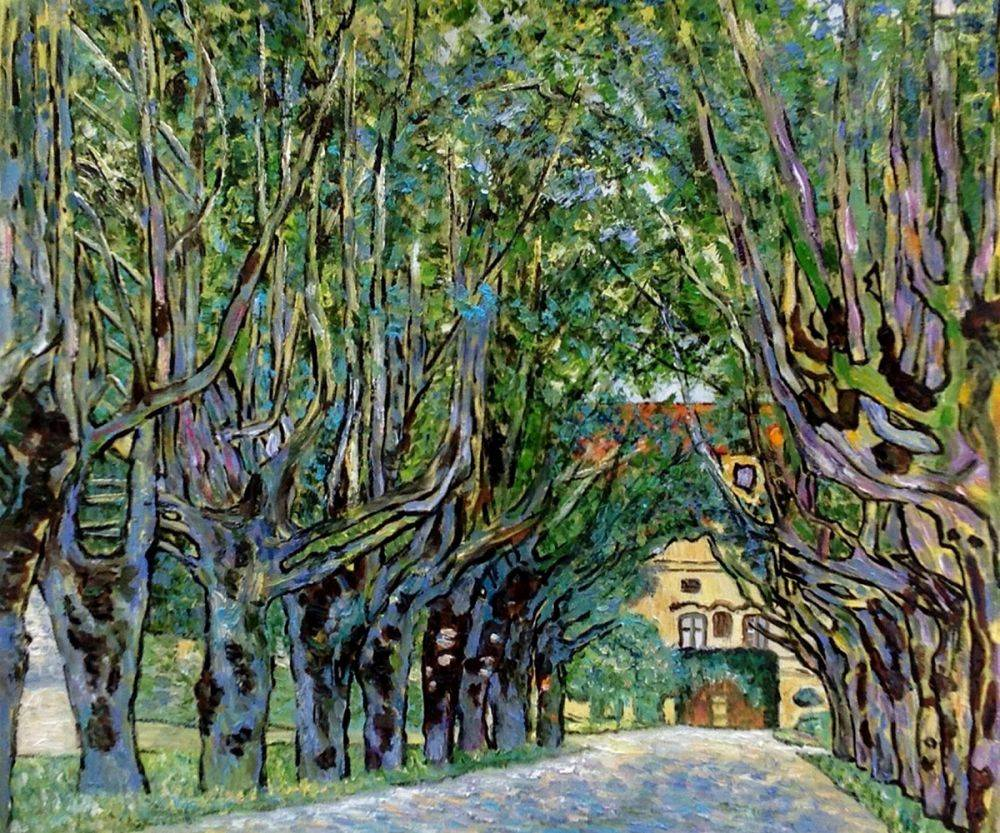
\includegraphics[width=\paperwidth]{../assets/Klimt_Kammer_1.jpg}}
%{../assets/forallx-beamer-background.pdf}}
\maketitle}

\begin{frame}
  \frametitle{Course components}

  \begin{itemize}[<+->]
  \item Textbook
  \item Lecture videos on D2L
  \item Synchronous Zoom sessions
  \begin{itemize}
    \item WF 12:00--12:50
  \end{itemize}
  \item Tutorials
  \begin{itemize}
    \item WF 9:00--10:50
  \end{itemize}
  \item D2L website \& discussion forums
  \item PASS Sessions
  \end{itemize}
\end{frame}

\begin{frame}
  \frametitle{Textbook}

  \begin{columns}
    \begin{column}{.3\textwidth}
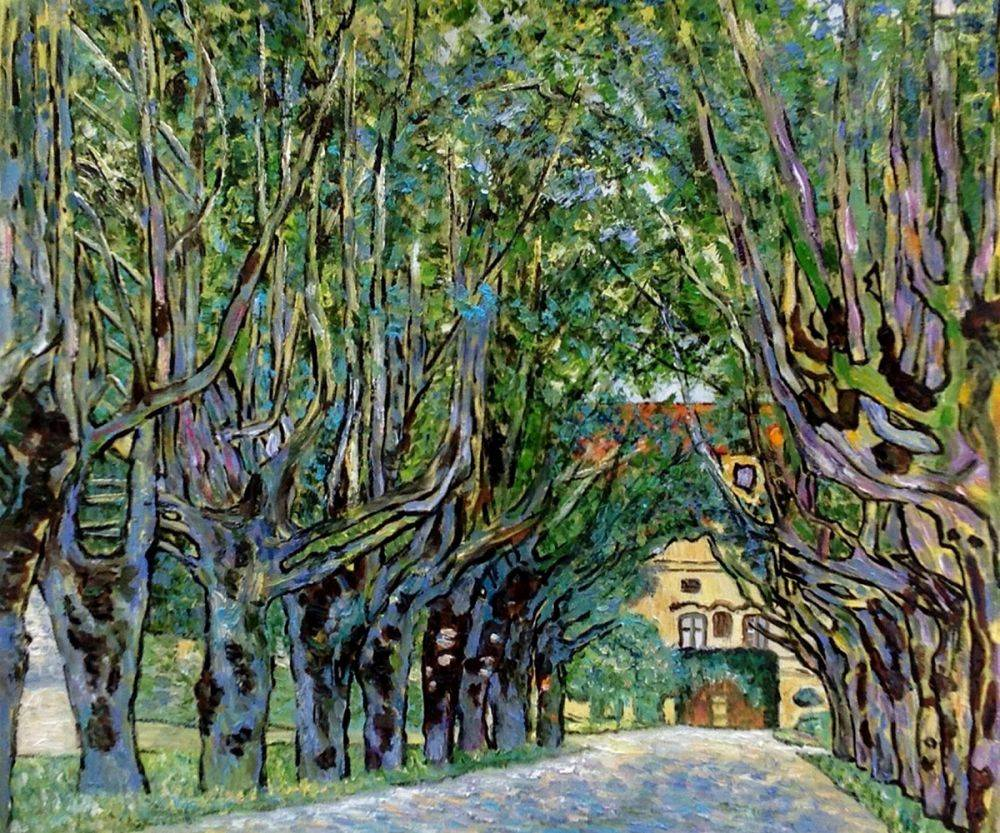
\includegraphics[height=.9\textheight]{../assets/Klimt_Kammer_1.jpg}
%{../assets/forallxyyc}
    \end{column}
    \begin{column}{.6\textwidth}
      \begin{itemize}
        \item Free!
        \item Available on D2L, and at\\ \href{https://forallx.openlogicproject.org/}{forallx.openlogicproject.org}
      \end{itemize}
    \end{column}
  \end{columns}
\end{frame}


\begin{frame}
  \frametitle{Problem sets}

  \begin{itemize}[<+->]
    \item Practice the material.
    \item Mostly online using \textit{Carnap} system.
    \item Collaboration ok.
    \item Should be done by Friday, will take till Monday midnight.
    \item Don't give away solutions.
  \end{itemize} 
\end{frame}

\begin{frame}
  \frametitle{Quizzes}

  \begin{itemize}[<+->]
    \item Online on D2L.
    \item Multiple choice, randomized questions.
    \item Open book, three attempts, untimed.
    \item Due Mondays at midnight.
    \item Test-like: must do them on your own.
  \end{itemize}
\end{frame}

\begin{frame}
  \frametitle{Timed problems}

  \begin{itemize}[<+->]
    \item Mostly online using \textit{Carnap} system.
    \item Open book, one attempt, timed.
    \item Due Mondays at midnight.
    \item Test-like: must do them on your own.
  \end{itemize}
\end{frame}

\begin{frame}{A typical week}

  \begin{description}[<+->]
    \item[Monday \& Tuesday] Watch videos, do reading reading.
    \item[Wednesday] Tutorials in the morning, lecture at noon.
        Start working on the problem set.
    \item[Thursday] Work on problem sets.
    \item[Friday] Tutorials in the morning, lecture at noon.
    Finish problem set.
    \item [Saturday--Monday] Complete the quiz and timed
    problem.
  \end{description}
\end{frame}

\begin{frame}{Grading philosophy}
  \begin{itemize}[<+->]
    \item We're using \emph{proficiency-based evaluation}.
    \item There are twelve weeks of material.
    \item Each week corresponds to one learning goal.
    \item You show proficiency in a learning goal by completing three
    assessments (problem set, quiz, timed problem).
    \item Your grade depends on \emph{how many} learning goals you complete.
    \item Ideally, you complete each goal during the week we cover it.
    \item But you get two chances to \emph{re-do assessments}.
  \end{itemize}
\end{frame}

\begin{frame}
  \frametitle{Completing assessments}

  \begin{itemize}[<+->]
    \item Each week covers one learning goal.
    \item Our aim is for you to achieve proficiency in these learning
    goals.
    \item Proficiency corresponds roughly to a B grade (``good performance'').
    \item Scoring 80\% or more on a
    problem set or quiz is ``complete.''
    \item Scoring 95\% or more is ``complete+'' (A-level,
    excellent performance).
    \item Timed problems are just complete/not complete: to meet
    the bar for a B, you have to submit a correct solution.
  \end{itemize}
\end{frame}

\begin{frame}{Earning your final grade}
  \begin{itemize}[<+->]
    \item For a B (good performance), you must complete (score at the level of a B) 10/12
    of each type of assessement (10 problem sets, 10 quizzes, 10
    timed problems).
    \item For an A (excellent performance), you must complete \emph{all} assessments and score complete+ on at least 10/12 quizzes and
    problem sets.
    \item For C, complete at least 8/12; and for a D, 6/12 of each assessment.
    \item For $+$ and $-$ grade criteria, see the outline.
  \end{itemize}
\end{frame}

\begin{frame}{Do-overs}
  \begin{itemize}[<+->]
    \item Multiple chances to show what you've learned.
    \item Immediate feedback on everything.
    \item Unlimited attempts on problem set questions.
    \item Three attempts on quizzes, no time limit.
    \item Only timed problems have time limits.
    \item Re-do timed problems or buy more attempts at quizzes using a token.
  \end{itemize}
\end{frame}

\begin{frame}{Tokens}
  Six tokens to spend on:
    \begin{itemize}[<+->]
      \item One more shot at a timed problem.
      \item Two day extensions in one week.
      \item Completing problem sets after deadline.
      \item Three more attempts on a quiz.
      \item Up to two do-overs per assessment.
    \end{itemize}
\end{frame}

\begin{frame}
  \frametitle{House rules}

  \begin{itemize}[<+->]
    \item Be civil and behave like adults: no sexist, racist, etc.
    jokes.
%    \item Don't distract others
%    \begin{itemize}
%      \item Phones to silent
%      \item Avoid use of devices for anything not related to class
%    \end{itemize}
  \item Collaborate and study together, but turn in only your own
  independent work.
  \item Don't give away answers.
  \item Don't cheat on quizzes and Timed Problems.
  \end{itemize}
\end{frame}

\begin{frame}
  \frametitle{Read the course outline!}

\begin{itemize}[<+->]
\item Official outline covers all policy questions.
\item Outline is binding agreement and you are responsible for knowing policies.
\item Available on D2L and Philosophy Department website.
\end{itemize}

%\bigskip
%\centerline{Questions?}
\end{frame}

\setbeamertemplate  {frame numbering}{\thesection.\thesubsection.\number\numexpr \insertframenumber-\subsecframestart}